\documentclass{article}
\usepackage[utf8]{inputenc}
\usepackage{graphicx}

\title{Ear and Hearing}
\author{MCB C61 with Professor David Presti \\ \\ Benjamin Lee}
% \date{21 March 2018}

\begin{document}

\maketitle


\textbf{Key Concepts:} 
\begin{itemize}
    \item Sound: Physical and Perceptual properties, frequency, amplitude, tone, pitch, loudness
    \item Human Hearing Range (frequency)
    \item Speed of Sound 
    \item Timbre
    \item Joseph Fourier and Fourier analysis 
    \item Cochlea, Basilar membrane, Fourier analysis
    \item Hair cells (inner and outer)
    \item Perception of one's own voice 
    \item Auditory Nerve
    \item Auditory Neural pathways into brain
    \item Primary Auditory Cortex, A1
    \item Hearing loss: infection, genetic, noise-induced
    \item Vestibular system
    \item Semicircular canals
    \item Utrile, saccule
    \item Otolith
\end{itemize}

\newpage
\section{Sound: Physical and Perceptual}
\textbf{Definition 1:} Sound is a \textbf{mental experience} and requires someone or something capable of mental experience as well as a \textbf{sound-detecting organ} (ear) according to our understanding. \\
\textbf{Definition 2:} Sound is a \textbf{variation in air pressure} generated by some action or source. \textbf{(physical vibration)} \\

These definitions are usually not a problem unless we are faced with problems such as the tree falling in the forest. \\

The mental experience of sound is generated by processes of the nervous system elicited by the physical stimulus of rhythmic air pressure variation, such as the action of a tree falling. When the tree falls, it \textbf{compresses} the air molecules (N and O, mainly) in the vicinity, producing a transient increase in their density. Increased \textbf{density} pushes on the nearby molecules, compressing them. Compression is followed by a \textbf{rebound of rarefaction} or thinning. The variation in air pressure moves out into the space around the falling tree as a wave of pressure variation, traveling at the \textit{speed of sound}. \\

\subsection{Frequencies}

\textbf{Sine Waves} are used to plot air pressure as a function of time \\

\noindent \textbf{Speed of Sound:} through air, sound moves at 1,100 feet per second (fps) (335 meters per second (mps) or 750 miles per hour (mph)) \\
Since velocity (feet/second) is equal to frequency of variation (cycle/second) multiplied by wavelength (feet/cycle), we can see that an air pressure at this velocity oscillating at 200 Hz has wavelength of 5.5 feet. \\
\begin{center}
Wave velocity = frequency * wavelength \\
1,100 feet/second = 200 cycle/second * 5.5 feet/cycle \\
\end{center}

\begin{itemize}
    \item The \textbf{higher} the frequency, the shorter the wavelength. Made of \textbf{faster pressure variations} which are experienced as sounds with high pitch or tone 
    \item The \textbf{shorter} the frequency, the longer the wavelength. \textbf{Slower pressure variations} are experienced as sounds having lower pitch or tone. 
\end{itemize}

\noindent \textbf{Loudness:} associated with the \textbf{amplitude} or magnitude of the pressure variation. High amplitude is louder than low amplitude. (size or height of the sine waves) \\

\noindent \textbf{Speed of Light:} 186,000 miles per second (300,000,000 meters per second) \\
Note: Speed of Light $>$ Speed of Sound (ex: see lighting first before we hear it)\\
Light can be conceptualized as a propagating vibration of an electromagnetic field. Corresponding to tone and loudness for sound are color and brightness for light respectively. \\

\noindent \textbf{Human Hearing Range:} 20 to 20,000 Hz \\ 
Note: For electromagnetic radiation, wavelength is the preferred unit of description \\
For sound, frequency is the preferred unit of description. But both can use either. \\

\subsection{Timbre}
Related to the complexity of the sound waveform. Complex waveforms are associated with mental experiences of sound having richness and complexity beyond that of pure tones. (Greek \textit{tympanon} = drum) \\
Musical intruments are perfect examples of timbre, although you may play a middle C on a piano it is still not a pure tone. \\ 

\textbf{Two tones:}
\begin{itemize}
    \item \textbf{Simple:} also known as pure tones. One simple frequency 
    \item \textbf{Complex:} mixture of several different frequencies. Combination of many simple tones and closer to actual air pressure variations. 
\end{itemize}

\newpage 
\section{Fourier Analysis}
Complex waveform describing a vibration can always be represented as a \textbf{sum of sine waves} having various frequencies and amplitudes \\
Known as a Fourier series, Fourier decomposition, or Fourier analysis named after French mathematician Joseph Fourier (1768-1830). \\ 

\noindent Useful in decomposing sound waves or combining sound waves. 

\section{Ear Structure}

\subsection{Outer Ear}
\begin{itemize}
    \item \textbf{Pinna:} Most external structure of the ear. Fleshy flap of skin on each side of the head. 
        \subitem Functions as funnel or antenna collecting and focusing the vibrations of air pressure into the ear canal. 
    \item \textbf{Eardrum:} (tympanic membrane) small drumskin-like piece of tissue that is set in vibration when air molecules strike it. Boundary between outer ear and middle ear.
\end{itemize}

\subsection{Middle Ear}
\begin{itemize}
    \item \textbf{Ossicles:} three small interconnected bones in a cavity of the middle ear. 
        \subitem Individually they are called the hammer, anvil, and sitrrup (Latin: \textit{malleus, incus,} and \textit{stapes})because of their shapes. 
        As eardrum vibrates, the hammer (attached to eardrum) vibrates. The vibrations transfer to the anvil and then the stirrup. Which is attached to the \textit{oval window}
    \item \textbf{Oval Window:} Boundary between middle ear and inner ear
\end{itemize}

\subsection{Inner Ear}
\begin{itemize}
    \item Consists of \textbf{Cochlea} and \textbf{Semicircular Canals} collectively called the bony labyrinth. 
    \item Interior of bony labyrinth is filled with fluid (water and ions) 
    \item Vibration of Oval window vibrates the fluid inside the cochlea. 
    \item Structure of \textit{ossicles} allows the vibrational energy to be efficiently transferred from medium of air into the medium of fluid
    \item Running the length of the cochlea, down the spiral interior, is a thin tissue called the \textit{basilar membrane}, which vibrates as the surrounding fluid vibrates
    \item \textbf{Basilar membrane} varies in thickness being most thick near the oval window and least at the other end. Thickness causes it to be set into vibration by different frequencies. Thicker end, higher frequencies. Thinner end, lower frequencies. 
    \subitem Creates a spatial representation of the component frequencies of sound entering the ear - a \textbf{Fourier analysis} of the sound
\end{itemize}

\begin{figure}[htp]
\centering
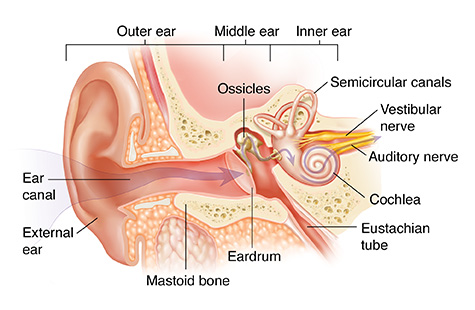
\includegraphics[width=8cm]{images/ear.png}
\caption{The Ear}
\label{fig: Ear}
\end{figure}

\subsection{Hair Cells}
Along the length of the basilar membrane are thousands of hair cells. Characterized by a bundle of hairs or cilia attached to one end. \\

\noindent As the basilar membrane vibrates the hair cells vibrate as well. The fluid surrounding the hairs or cilia swoosh them back and forth detecting different signals. \\
The hair cell has chemical synapses with fibers of the auditory nerve, \textbf{cranial nerve 8}. The bending of the hairs initiates a sgnal from the hair cell to the brain. \\

\begin{figure}[htp]
\centering
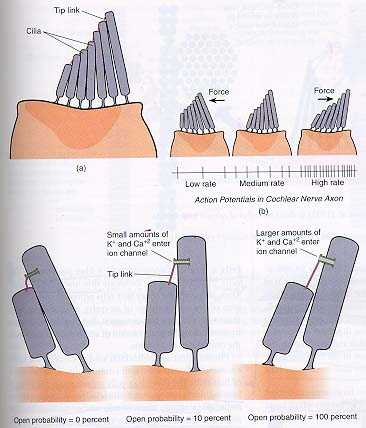
\includegraphics[width=7cm]{images/haircells.jpg}
\caption{Hair Cells}
\label{fig: Hair cells}
\end{figure}

\textbf{How the Neural Signal is Generated:}
\begin{itemize}
    \item Hairs interconnected by tiny molecular cables (few billionths of a meter in diameter)
    \item Tiny cables appear to be coupled to positive ion channels, so as hairs bend, cables tug on channels to open them
    \item When channels open, K$^+$ ions (in cochlear fluid K$^+$ more concentrated outside cells than inside) flow into the hairs and make the normally negative interior of the hair cell more positive
    \item Depolarization of the hair cell's membrane potential causes voltage-gated calcium channels to open and Ca$^++$ ions flow into the cell
    \item Influx of Ca$^{++}$ triggers fusion of synaptic storage vesicles with outer membrane of the cell, release of neurotransmitter molecules released into synaptic cleft. 
    \item Activates postsynaptic receptors on dendritic fiber of auditory nerve. If enough stimulation, action potential occurs and signal is sent to brain. 
\end{itemize}

\subsection{Perception of one's own Voice}

Direct vibration of the bones of the skull that surround the cochlea cause sound in the inner ear as well. 
Vibrates the tympanic membrane, ossicles, and cochlea. \\

\noindent We perceive our voices both externally and internally, which is why our own voice sounds different when we record it and just hear our pure voice without the vibration of our skull. The frequency of vibrations that propagate through air space differ from from vibrations that propagate through our bones and other body parts. \\

\newpage
\section{Auditory Nerve} 

\textbf{Auditory Neural pathways into brain:}
\begin{itemize}
    \item Auditory signaling: neurotransmitter is released from hair cell and signal sent to postsynaptic dendrite of cranial nerve 8
    \item Cell bodies of thees located in a cluster called the spiral ganglion (one cluster for each ear) 
    \item Called \textbf{bipolar neurons} with a single myelinated dendrite receiving the signal from the hair cell and a myelinated axon carrying the signal into the brainstem. 
    \item In brainstems \textbf{medulla}, axons of auditory nerve synapse with cells in \textbf{cochlear nucleus}. 
        \subitem Neurons of the cochlear nucleus send axons to cells in regions of the pons called the \textbf{superior olive} and the \textbf{lateral lemniscus}
    \item Brainstem auditory centers all send axons to cells into the \textbf{inferior colliculus} in midbrain 
    \item Inferior colliculus  projects to the \textbf{medial geniculate nucleus (MGN)} of the \textbf{thalamus}
    \item MGN sends axons to \textbf{primary auditor cortex (A1)} in \textbf{temporal lobe}
\end{itemize}

Bilateral connectivity (mass interconnectivity on both sides of brain) allows us to detect location of sounds by comparing qualities of arrival times and sounds. \\

\noindent \textbf{Inner Hair Cells:} send signals to spiral ganglion and cochlear nucleus. 3,500 cells per cochlea. \\

\noindent \textbf{Outer Hair Cells:} make fewer connections to spiral ganglion but receive much more efferent input from the brainstem. 12,000 cells per cochlea. \\
Main function to change sensitivity of basilar membrane, making it more sensitive to low sounds. \textbf{Prestin} protein elongates and contracts as a function of membrane potential changes. Pushes against the basilar membrane to change its stiffness and sensitivity. 

\newpage
\section{Loss of Hearing}
Can be caused by infections, genetic anomalies and noise-induced. \\

\noindent \textbf{Infections} in the inner ear can cause irreversible damage to hair cells.\\

\noindent \textbf{Genetic Anomalies} can result in the malfunction of the cochlea.\\
One such anomaly involves a gene coding for a connexon ion channel protein, of the same type as those forming electrical synapses between neurons and glia. Connexon channels maintain ion flow between various chambers of the cochlea. Mutation in the gene coding for a particular channel in the cochlea, known as connexin 26, produces abnormal ion balances within the cochlea, resulting in deafness as the hair cells cannot function. \\

\noindent Most common cause of hearing loss is \textbf{acoustic Trauma}, exposure to loud sounds. \\
\textbf{Decibels (dB)} is the standard way of measuring sound intensity (loudness). In honor of Alexander Graham Bell (1847-1922).  \\
Defnining feature of decibel scale is it is logarithmic scale relative to a reference. \\
Anything higher than 85 decibals can potentially damage the hearing. Hearing damage thought to be caused by intense overstimulation of hair cells. Excitotoxic overstimulation can cause the death of hair cells as with brain cells in seizures. \\

Hearing aids can help hearing loss, as it amplifies the sound and projects it into the ear. (Ear trumpets to electronic to cochlear implants) \\ 

\newpage
\section{Vestibular System}

\textbf{Semicircular Canals:} three orthogonal (perpendicular and 90 degree angles to one another) canals in the bony labyrinth together with two bulbous cavities called the \textbf{utricle} and the \textbf{saccule}. \\

These sensory structures of the vestibular system help detect our \textbf{orientation} relative to gravity and our acceleration as we move, walk, and turn. Allows us to \textbf{maintain balance} and execute smooth and coordinated movement. \\

\noindent \textbf{Utricle} and \textbf{Saccule} are receptor cells that detect movement of fluid in the attached semicircular canals. The three orthogonal canals allow us to gather complete info about how the head is orientated and acceleration in the 3D world. Fluid moves around ear, detected by hair cells and neural signals are generated and passed to \textbf{cranial nerve 8}, which sends\textbf{ vestibular} as well as \textbf{auditory} info to the brain. \\

\noindent \textbf{Otoliths:} ear stones. Tiny microscopic stones, crystals of calcium carbonate found in vestibular hair cells.\\

Inertia of these stones contribute to bending of hairs in sensory cells. Contribute to generating and amplifying the sensory signals that allow us to maintain balance as we move. \\

Out of our conscious awareness except for dizziness and vertigo (caused by inflammation or infection of vestibular system). \\
\end{document}